\documentclass{jsarticle}

\usepackage[dvipdfmx]{graphicx}

\usepackage{bm}

\def\N{{\mathcal{N}}}
\def\w{{\bm{w}}}
\def\p{{\bm{\phi}}}
\def\D{{\mathcal{D}}}
\def\t{{\mbox{\bf t}}}
\def\x{{\mbox{\bf x}}}
\def\T{{\mbox{T}}}
\def\S{{\mbox{\bf S}}}
\def\I{{\mbox{\bf I}}}

\def\size{1000}

\begin{document}


\section{ベイズの復習}

\begin{eqnarray*}
  p(\w, \D)  & = & p(\D)p(\w|\D) = p(\w)p(\D|\w) \\
  p(\w|\D) & = & \frac{p(\D|\w)p(\w)}{p(\D)}
\end{eqnarray*}

\section{1.2.6 ベイズ曲線フィッティング}

\begin{figure}
  \centering
  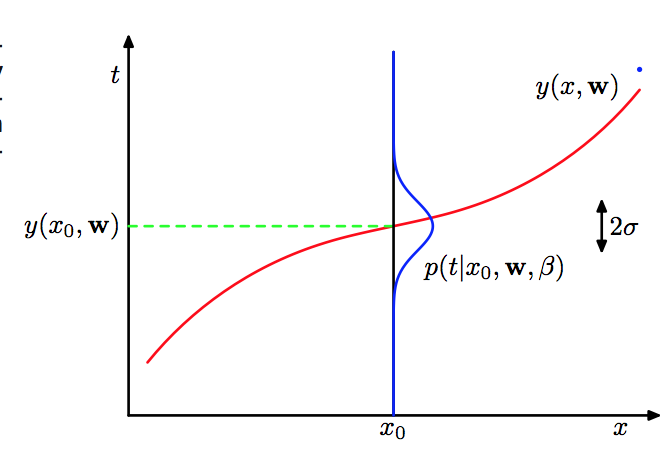
\includegraphics[width=0.8\textwidth]{f1-16.png}
  \caption{1.18}
\end{figure}

\begin{eqnarray*}
p(\w|\x,\t, \alpha,\beta) & = & \frac{p(\t | \x,\w,\beta) p(\w|\alpha)}{p(\x,\t, \alpha, \beta)} \\
  p(\w|\x,\t, \alpha,\beta) & \propto & p(\t | \x,\w,\beta) p(\w|\alpha) \ \ \ \ \ \ \ (1.66)
\end{eqnarray*}
上記は、最大事後確率(MAP; maximum a posteriori)となるが、最大となる{\bf w}の点を推定しているだけ。完全なベイズというには{\bf w}のすべての値で積分する必要がある。(すなわち、いろいろな$w$がそれぞれの事後確率で出力され、それぞれの$w$にて$x$から$t$を予想する)。問題としては、$x$から$t$を予測する問題で、訓練例として$\x,\t$が与えられるので次のようになる。
\begin{equation}
  p(t|x,\x,\t) = \int p(t|x,\w) p(\w|\x,\t)d\w \ \ \ \ \ \ \ \ (1.68)
\end{equation}
ここで式(1.60)から、
\[
p(t|x,\w,\beta)  = \N(t|y(x,\w),\beta^{-1}) \ \ \ \ \ \ \ \ (1.60)
\]
\[
p(t|x,\t)  = \N(t|y(x,\w)) \ \ \ \ \ \ \ \ (1.60')
\]
式(1.66)から、事後分布
\[
p(\w|\x,\t) = \frac{p(\t | \x,\w,\beta) p(\w|\alpha)}{\sum p(\t | \x,\w,\beta) p(\w|\alpha)}
\]

となり、これらから、式(1.68)は解析的に解くことができ、
\[
p(t|x,\x,\t) = \N(t|m(x),s^2(x))  \ \ \ \ \ \ \ \ (1.69)
\]
ここで、平均と分散は、
\begin{eqnarray*}
  m(x) & = &\beta\p(x)^{\T}\S\sum_{n=1}^{N}\phi(x_n)t_n \ \ \ \ \ (1.70) \\
  s^2(x) & = & \beta^{-1} + \p(x)^{\T}\S\p(x) \ \ \ \ \ (1.71)
\end{eqnarray*}
となり行列$\S$は、
\begin{eqnarray*}
  S^{-1} = \alpha\I+\beta\sum_{n=1}^{N}\p(x_n)\p(x_n)^\T
\end{eqnarray*}
で与えられる。ここで$\I$は単位行列で、$\phi_i(x) = x^i (i=0,...,M)$

\begin{figure}
  \centering
  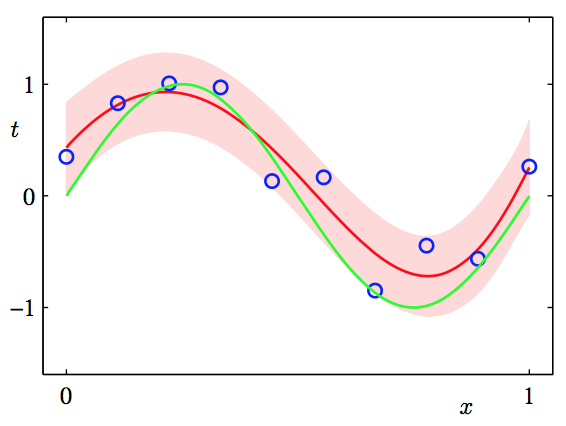
\includegraphics[width=0.8\textwidth]{f1-17.png}
  \caption{1.17}
\end{figure}

\section{1.3 モデル選択}

最小二乗法の例にて、最適な次数があった。
次数のようなモデルの複雑さを、最小二乗法では正則化係数$\lambda$により制御するし、他の学習手法もそのようなパラメータがある。これらは未知の事例に対する予測が最も良いものを選びたい。

過学習があるので、訓練データとは別に、{\bf 確認用集合(検証用集合; validation set)}を用意しておき、これらのパラメータを調整し、最後に、{\bf テスト用集合(test set)}にて性能の最終評価を行う。

\begin{itemize}
\item 交差確認(交差検証; cross-validation) 訓練集合を$S$個に分割し、$(S-1)/S$の割合部分を訓練に使いつつ残りの$1/S$の割合部分のデータで性能の評価に用いることを、$S$通り行う。
\item LOO法(1個抜き法; leave-one-out method)上記の割合を1事例毎にしたもの。\footnote{ジャックナイフ法ともよばれる。}
\end{itemize}
欠点は計算時間がかかる。

\begin{figure}
  \centering
  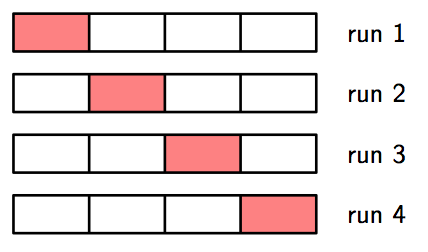
\includegraphics[width=0.8\textwidth]{f1-18.png}
  \caption{1.18}
\end{figure}

情報量基準(information criterion)というバイアスに対するペナルティ。
\begin{itemize}
\item 赤池情報量基準(AIC)
  \[
  \ln p(\D | \w_{\mbox{ML}})-M
  \]
  ここで$p(\D | \w_{\mbox{ML}})$は対数尤度である。
\item ベイズ情報量基準(BIC) 4.4.1節。
\item 3.4節では完全なベイズアプローチ
\end{itemize}

\end{document}


